%
%	Configure LaTeX to produce a PDF "book" using the memoir class
%

\documentclass[10pt,oneside]{memoir}

%
%	Generic Configuration for memoir-based documents
%

\usepackage{layouts}[2001/04/29]


% In case we need a glossary, or index
\usepackage[acronym]{glossaries}
\glstoctrue
\makeglossaries
\makeindex


% Basic page layout configuration
\def\mychapterstyle{default}
\def\mypagestyle{headings}


% Use 8.5 x 11 inch page layout
%
%	8.5 x 11 layout for memoir-based documents
%


%%% need more space for ToC page numbers
\setpnumwidth{2.55em}
\setrmarg{3.55em}

%%% need more space for ToC section numbers
\cftsetindents{part}{0em}{3em}
\cftsetindents{chapter}{0em}{3em}
\cftsetindents{section}{3em}{3em}
\cftsetindents{subsection}{4.5em}{3.9em}
\cftsetindents{subsubsection}{8.4em}{4.8em}
\cftsetindents{paragraph}{10.7em}{5.7em}
\cftsetindents{subparagraph}{12.7em}{6.7em}

%%% need more space for LoF numbers
\cftsetindents{figure}{0em}{3.0em}

%%% and do the same for the LoT
\cftsetindents{table}{0em}{3.0em}

%%% set up the page layout
\settrimmedsize{\stockheight}{\stockwidth}{*}	% Use entire page
\settrims{0pt}{0pt}

\setlrmarginsandblock{1.5in}{1.5in}{*}
\setulmarginsandblock{1.5in}{1.5in}{*}

\setmarginnotes{17pt}{51pt}{\onelineskip}
\setheadfoot{\onelineskip}{2\onelineskip}
\setheaderspaces{*}{2\onelineskip}{*}
\checkandfixthelayout


% Use default packages for memoir setup
%
%	Default packages for memoir documents created by MultiMarkdown
%

\usepackage{fancyvrb}			% Allow \verbatim et al. in footnotes
\usepackage{graphicx}			% To enable including graphics in pdf's
\usepackage{booktabs}			% Better tables
\usepackage{tabulary}			% Support longer table cells
\usepackage[T1]{fontenc}		% Use T1 font encoding for accented characters
\usepackage[utf8]{inputenc}		% For UTF-8 support
\usepackage{xcolor}				% Allow for color (annotations)
\usepackage{listings}			% Allow for source code highlighting
\usepackage[sort&compress]{natbib} % Better bibliography support
\usepackage[normalem]{ulem}		% Support strikethrough

\input{mmd6-criticmarkup}



% Configure default metadata to avoid errors
%
%	Configure default metadata in case it's missing to avoid errors
%

\def\myauthor{Author}
\def\defaultemail{}
\def\defaultposition{}
\def\defaultdepartment{}
\def\defaultaddress{}
\def\defaultphone{}
\def\defaultfax{}
\def\defaultweb{}
\def\defaultaffiliation{}

\def\mytitle{Title}
\def\subtitle{}
\def\mykeywords{}


\def\bibliostyle{plain}
% \def\bibliocommand{}

\def\myrecipient{}

% Overwrite with your own if desired
%\input{ftp-metadata}






\def\mytitle{churn}
\def\myauthor{Nguyen Tam}
%
%	Get ready for the actual document
%

\usepackage[
	plainpages=false,
	pdfpagelabels,
	pdftitle={\mytitle},
	pagebackref,
	pdfauthor={\myauthor},
	pdfkeywords={\mykeywords}
	]{hyperref}
\usepackage{memhfixc}


%
%	Configure information from metadata for use in title
%

\ifx\latexauthor\undefined
\else
	\def\myauthor{\latexauthor}
\fi

\ifx\subtitle\undefined
\else
%	\addtodef{\mytitle}{}{ \\ \subtitle}
	\expandafter\def\expandafter\mytitle\expandafter{\mytitle \\ \subtitle}
\fi

\ifx\affiliation\undefined
\else
%	\addtodef{\myauthor}{}{ \\ \affiliation}
	\expandafter\def\expandafter\myauthor\expandafter{\myauthor \\ \affiliation}
\fi

\ifx\address\undefined
\else
%	\addtodef{\myauthor}{}{ \\ \address}
	\expandafter\def\expandafter\myauthor\expandafter{\myauthor \\ \address}
\fi

\ifx\phone\undefined
\else
%	\addtodef{\myauthor}{}{ \\ \phone}
	\expandafter\def\expandafter\myauthor\expandafter{\myauthor \\ \phone}
\fi

\ifx\email\undefined
\else
%	\addtodef{\myauthor}{}{ \\ \email}
	\expandafter\def\expandafter\myauthor\expandafter{\myauthor \\ \email}
\fi

\ifx\event\undefined
\else
	\date[\mydate]{\today}
\fi

\ifx\latextitle\undefined
	\def\latextitle{\mytitle}
\else
\fi

\title{\mytitle}
\author{\myauthor}

\ifx\mydate\undefined
\else
	\date{\mydate}
\fi


\ifx\theme\undefined
\else
	\usetheme{\theme}
\fi

\begin{document}

\VerbatimFootnotes


\chapterstyle{\mychapterstyle}
\pagestyle{\mypagestyle}

% Frontmatter
\frontmatter

% Title Page
\maketitle
\clearpage

%
% Copyright Page
%

\vspace*{\fill}
\setlength{\parindent}{0pt}

\ifx\mycopyright\undefined
\else
	\textcopyright{} \mycopyright
\fi

\begin{center}
	\framebox{ \parbox[t]{1.5in}{\centering Formatted for \LaTeX \\ 
	by MultiMarkdown 6}}
\end{center}

\setlength{\parindent}{1em}
\clearpage

\tableofcontents
%\listoffigures
%\listoftables


\mainmatter



\part{Introduction \#}
\label{introduction}

The telecommunication industry

The telecommunication industry consists of internet providers and telecommunication services, and it one of the largest industries in the information society. The traditional source of revenue for telecommunication industry has been callings, but it's changing to be texting, image and video processing due to the decreasing cost of accessing internet.

There are some characteristics of the telecom industry:

\begin{itemize}
\item It has heavy regulations by the governmental authorities (why).

\item The market is highly competitive with different providers trying to provide the same service. Therefore, prices tend to decrease over time.

\item Because there are large number of users national wide for the telecom and internet services, the amount of data gathered from customers by these providers is huge. Knowing how to extract valuable information from the customers can help telecom companies gain competitive edges against other competitors in the industry.

\end{itemize}

Customer churn is defined as the rate of customers quitting a service, and is one of the main issues in industries like telecommunications, internet service providers, e-commerce, marketing, and banking. The telecommunication industry particularly suffers the highest rate in any industry. Companies often focus on retaining customers rather than acquiring new ones because the cost of acquiring new customers can be five to six times higher than retaining existing customers (Colgate \& Danaher, 2000). In the telecommunication industry specifically, the market is saturated, making it difficult to attract new customers (Manďák, 2018). On the customer side, it is very easy for customers to switch to a new provider if it provides a more beneficial offer (Canale and Lunardon, 2014). Therefore, it is important to invest in developing customers' trust and loyalty for the service. Having an understanding of the influential factors causing customer churn can help companies understand customers' needs and adjust on their provided services to reduce churn.

Churn is an important part of the Customer Relationship Management (CRM). In CRM, the core concepts of customer equity entails customer retention and is one of the most important component of the customer lifetime value framework applied in marketing and other business applications. From an analytical perspective, the period of which a customer remain at the service is essential for companies to calculate lifetime value (CLV) and customer equity, since this rate drives companies' profits and growth. While companies acknowledge its importance, not many companies are successful at retaining their customers. 85\% customers think companies could do more to keep them. 49\% of managers in companies report not satisfied with their customer retention goal. More researches also report retention campaigns can cause harm instead of attaining the intended goal.

\part{Method \#}
\label{method}

Why doesn't this project use other modeling approaches
There are approaches which focus on the predictive modeling such as the predictive modeling approach used by Max Kuhn. This approach focuses in detail how a machine learning pipeline works, and will dive deep into the details of the decisions in modeling. Though this approach has certain benefits in helping us detailing the decisions made when conducting models, we instead use a more business-oriented framework, which is called the CRISP Framework.
Benefits of the CRISP Framework
CRISP helps to build a data science project based on business results and financial benefits. I will follow this framework since it combines both the data science approach and the evaluation of the project. It connects the models with the return on investment to show the value or impact from the business. The reasons we also use CRISP is because:

\begin{itemize}
\item It's an agile method: it implements data science projects iteratively, helping us to overcome common sense thinking and help us to adjust to unexpected issues quickly.

\item It's data science for business's sake. It focuses on the ROI of the project, helping us to evaluate KPIs and potential economic impact if the model is implemented. It also ensures that we always iterate our projects to meet the business goal.

\end{itemize}

In terms of churn, ROI is one of the most critical metrics in which we want to know besides the technical aspect of data science. Follow this framework step-by-step helps us to make sure we don't miss any important steps during the processIt allows us to focus on processes that require human involvement that requires creativity and intelligence, parts that have not been automated by machines.

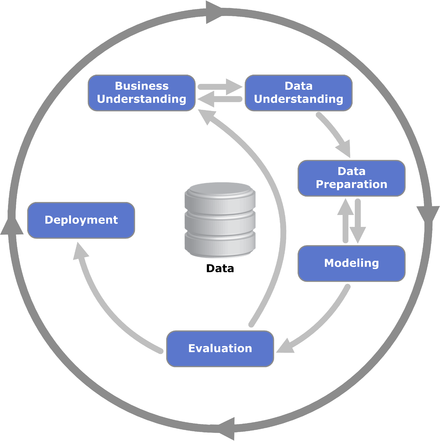
\includegraphics[width=333pt,height=334pt]{CRISP.png}
The CRISP Framework

%
%	MultiMarkdown default footer file
%


% Back Matter
\if@mainmatter
	we're in main
	\backmatter
\fi


% Bibliography

\ifx\bibliocommand\undefined
\else
	\bibliographystyle{\bibliostyle}
	\bibliocommand
\fi



% Glossary
\printglossaries


% Index
\printindex


\end{document}
